\documentclass{article}
\usepackage{hyperref}
\usepackage[table]{xcolor}
\usepackage{listings}
\usepackage{lmodern}
\usepackage[left=0.25in, right=0.25in, top=0.75in, bottom=0.75in]{geometry}
\usepackage{graphicx}
\usepackage{amsmath,amssymb}
\usepackage{tikz}
\usepackage{pgfplots}
\usepackage{subfigure}
\usepackage{enumerate}
\usepackage{tcolorbox}
\usepackage{fancyhdr}
\usepackage{cancel}
\usepackage{placeins}
\usepackage{multirow}
\usepackage{algorithm2e}
\usepackage{booktabs}
\usepackage{bbding}
\pagecolor{white}
\color{black}

\pagestyle{fancy}

\hypersetup{%
  colorlinks=true,% hyperlinks will be black
  linkbordercolor=red,% hyperlink borders will be red
  pdfborderstyle={/S/U/W 1}% border style will be underline of width 1pt
}

\newcommand{\soln}{\\ \textbf{Solution}: }
\newcommand{\bkt}[1]{\left(#1\right)}

\lhead{MA5892: Numerical Methods and Scientific Computing}
\chead{Assignment: 4}
\rhead{Roll number: PH15M015}

\begin{document}
\begin{enumerate}
\item Compute $\displaystyle \int_{0}^{1} e^{x^{2}} \ dx$ using the trapezoidal rule and 
trapezoidal rule with end corrections using the first and third derivatives. Perform this
by subdividing $[0, 1]$ into $N \in \{2, 5, 10, 20, 50, 100, 200, 500, 1000\}$ panels and 
plot the decay of the absolute error using the \textbf{three methods}. The value of the 
integral accurate upto $16$ digits is $1.4626517459071816$.

\textbf{Program:}
\lstinputlisting[language=Octave]{/home/saran/NMSC/Assignment/Assignment4/Octave/program.m}

%figure_1
\begin{figure}[ht!]
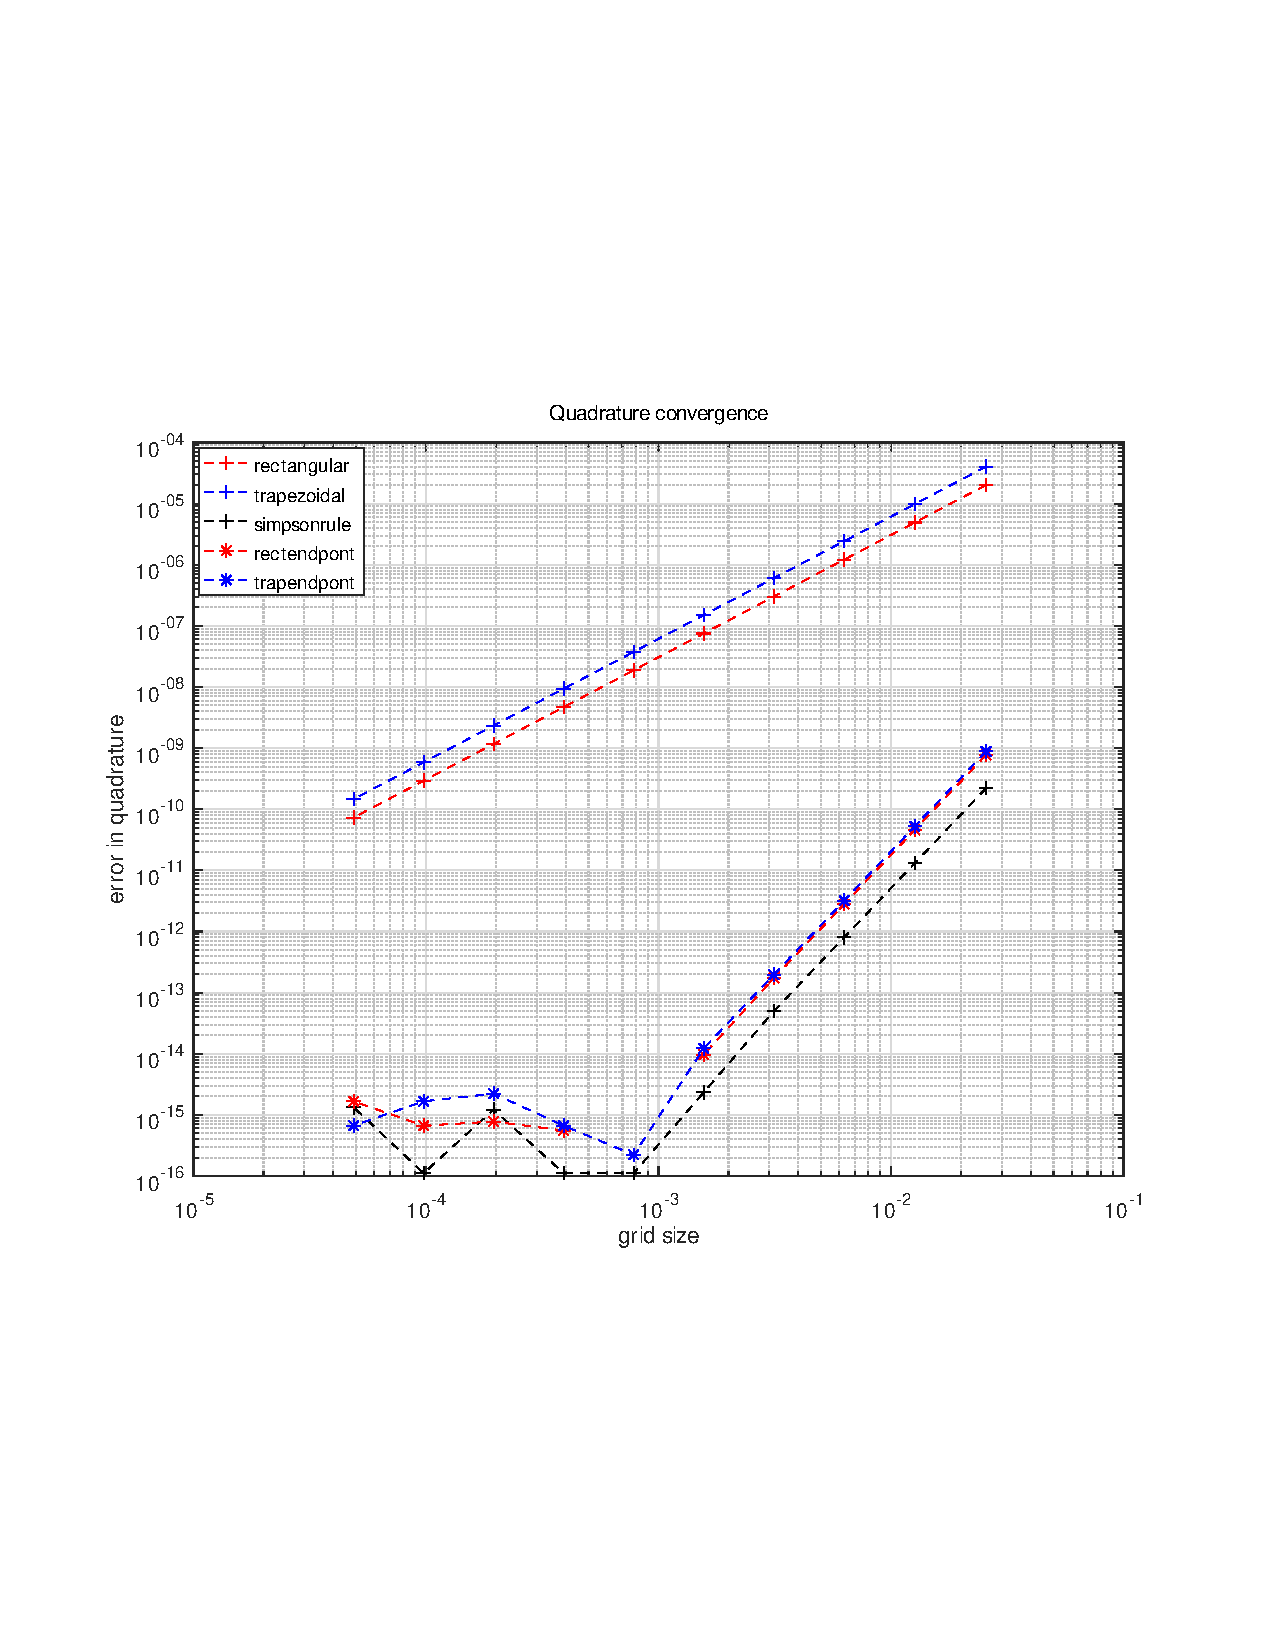
\includegraphics[width=30cm,height=20cm,keepaspectratio]{Octave/quadrature.pdf}
\centering
\end{figure}


\item Use the Euler-Macluarin to obtain
\begin{equation*}
\log (n!) = \log \displaystyle \left(C \left(\frac{n}{e} \right)^{n} \sqrt{n} \right) 
    + \mathcal{O}(1/n)
\end{equation*}
where $C$ is some constant. 

\textbf{Solution:}

The Euler-Maclaurin summation formula:
        \begin{equation}
            \displaystyle \sum_{n=0}^{\infty} f(x + n) = \displaystyle \int_{x}^{\infty}
            f(x)\ dx + \frac{1}{2} f(x) - \displaystyle \sum_{n=2}^{\infty}
            \frac{B_{n}}{n!} \frac{d^{n-1} f(x)}{dx^{n-1}}
        \end{equation}

It can be rewritten for the case of a finite sum as following:

        \begin{align}
            \displaystyle \sum_{k=n}^{N} f(k) &= \displaystyle \sum_{k=n}^{\infty} f(k) - \displaystyle \sum_{k=N+1}^{\infty} f(k) \\
            &= \displaystyle \sum_{k=n}^{\infty} f(k) - \displaystyle \sum_{k=N}^{\infty} f(k) + f(N) \\
            &= \displaystyle \sum_{k=0}^{\infty} f(k+n) - \displaystyle
            \sum_{k=0}^{\infty} f(k+N) + f(N) \\ 
            &= \displaystyle \int_{n}^{\infty} f(x)\ dx - \displaystyle \int_{N}^{\infty} f(x)\ dx + \frac{1}{2} f(n) - \frac{1}{2} f(N) + f(N) + \displaystyle \sum_{n=2}^{\infty} \frac{B_{n}}{n!} \frac{d^{n-1} f(n)}{dx^{n-1}} + \displaystyle \sum_{n=2}^{\infty} \frac{B_{n}}{n!} \frac{d^{n-1} f(N)}{dx^{n-1}} \\
            &= \displaystyle \int_{n}^{N} f(x)\ dx + \frac{1}{2} \left[f(n) + f(N)\right]
            + \displaystyle \sum_{n=2}^{\infty} \frac{B_{n}}{n!} \left[\frac{d^{n-1}
            f}{dx^{n-1}}\bigg|_{x=N} - \frac{d^{n-1} f}{dx^{n-1}}\bigg|_{x=n} \right]
        \end{align}

        let's consider the Stirling's approximation for $\Gamma(n)$ for positive integer
        $n\gg1$

        \begin{equation}
            \Gamma(n+1) = n!
        \end{equation}

        \begin{equation}
            \ln(\Gamma(n+1)) = \ln n! = \ln (1 \cdot 2 \cdot 3 \cdot ... \cdot (n-1) \cdot n) = \displaystyle \sum_{k=1}^{n} \ln k
        \end{equation}

The first two terms in Eq.(6) give us the following approximation:

\begin{equation*}
    \ln(\Gamma(n+1)) &= \ln(n!) = \displaystyle \int_{1}^{n} \ln(x)\ dx + \frac{1}{2} (\ln(1) + \ln(n)) \\
    &= x \ln(x)\bigg|_{1}^{n} - \displaystyle \int_{1}^{n} \frac{x}{x}\ dx + \frac{1}{2} \ln(n) \\
    &= n \ln(n) - n + 1 + \frac{1}{2} \ln(n)
\end{equation*}

Let's notice first that the term with the derivatives of $\ln(x)$ at $x=n$ in Eq.(6) are
proportional to negative powers of $n$ and thus $\rightarrow 0$ as $n \rightarrow \infty$.
On the other hand, the sum of the term with the derivatives of $\ln(x)$ at $x=1$ is a
constant independent of $n$. Thus, 

\begin{align*}
    \ln \Gamma(n+1) &= \ln n!  \\
                    &= \ln \left(\frac{n}{e}\right)^{n} + \ln \sqrt{n} + \ln(C) \\
                    &= \ln \left(C \sqrt{n} \left(\frac{n}{e}\right)^{n}\right)
\end{align*}

\item We will now determine $C$ in the above question as follows.
\begin{itemize}
    \item Use integration by parts to obtain an expression for $I_{k} = \displaystyle
        \int_{0}^{\pi/2} sin^{k}(x)\ dx$ (It might be easier to look at the even and odd
        cases separately)

    \item Prove that $I_{k}$ is a monotone decreasing sequence.

    \item Show that
        \begin{equation*}
            \lim_{m \to \infty} \frac{I_{2m - 1}}{I_{2m + 1}} = 1
        \end{equation*}

    \item Conclude that
        \begin{equation*}
            \lim_{m \to \infty} \frac{I_{2m}}{I_{2m + 1}} = 1
        \end{equation*}

    \item Hence, infer that the central binomial coefficient is asymptotically given by
        \begin{equation*}
            \binom{2m}{m} \sim \frac{4^{m}}{\sqrt{m\pi}}
        \end{equation*}
        where $f(m) \sim g(m) \Longrightarrow \lim_{m \to \infty} \displaystyle
        \frac{f(m)}{g(m)} = 1$

    \item Conclude that $C$ in the above question is $\sqrt{2\pi}$

    \item Hence, obtain the Stirling formula:
        \begin{equation*}
            n! \sim \left(\frac{n}{e}\right)^{n} \sqrt{2\pi n}
        \end{equation*}

    \item Obtain the relative error in $n!$ using the Stirling formula for $n \in \{20,50\}$

    \item Obtain a better estimate for $n!$, which is accurate upto $\mathcal{O}(1/n^{3})$
\end{itemize}

\end{enumerate}
\end{document}
